\begin{proof}
    First I can write the Lagrangian function for the problem (the sum of the objective function and the weighted constraints):
    \[L(x,y,\mu_1,\mu_2) = (x-a)^2+(y-b)^2+xy + \mu_1(x-1) + \mu_2(y-2)\]
    The Kuhn-Tucker conditions (which are necessary, but not sufficient, for a point to be a minimum) are:
    \begin{gather}
        2(x-a) + \mu_1 + y \geq 0 \label{KKT1} \tag{KKT1} \\
        2(y-b) + \mu_2 + x \geq 0 \label{KKT2} \tag{KKT2} \\
        x[2(x-a) + \mu_1 + y] = 0 \label{KKT3} \tag{KTT3} \\
        y[2(y-b) + \mu_2 + x] = 0 \label{KKT4} \tag{KKT4} \\
        x \geq 0 \label{KKT5} \tag{KKT5} \\
        y \geq 0 \label{KKT6} \tag{KKT6} \\
        x - 1 \leq 0 \label{KKT7} \tag{KKT7} \\
        y - 1 \leq 0 \label{KKT8} \tag{KKT8} \\
        \mu_1(x - 1) = 0 \label{KKT9} \tag{KKT9} \\
        \mu_2(y - 1) = 0 \label{KKT10} \tag{KKT10} \\
        \mu_1 \geq 0 \label{KKT11} \tag{KKT11} \\
        \mu_2 \geq 0 \label{KKT12} \tag{KKT12} 
    \end{gather}
    In order to find the points that satisfy these conditions, I have to explore various cases. Specifically, both the \eqref{KKT9} and \eqref{KKT10} must be true. It follows that:
    \[(\mu_1 = 0 \lor x = 1) \land (\mu_2 = 0 \lor y = 1)\]
    \begin{enumerate}
        \item \(\mu_1 = 0 \land \mu_2 = 0\)\par
            In order to find values for \(x\) and \(y\), I can use \eqref{KKT3} and \eqref{KKT4}, together with the values \(\mu_1 = 0\) and \(\mu_2 = 0\):
            \[
                \begin{cases}
                    x[2(x-a) + y] = 0 \\
                    y[2(y-b) + x] = 0
                \end{cases}
            \]
            I can now try to solve the system. Some possible solutions are easy to find:
            \begin{gather}
                \mu_1 = 0, \mu_2 = 0, x = 0, y = 0 \label{SOL1} \tag{SOL1} \\
                \mu_1 = 0, \mu_2 = 0, x = 0, y = b \label{SOL2} \tag{SOL2} \\
                \mu_1 = 0, \mu_2 = 0, x = a, y = 0 \label{SOL3} \tag{SOL3}
            \end{gather}
            I can now assume that neither \(x\) nor \(y\) is \(0\).
            \[
                \begin{cases}
                    x[2(x-a) + y] = 0 \\
                    y[2(y-b) + x] = 0
                \end{cases}
            \]
            \[
                \begin{cases}
                    y = \frac{2x(a-x)}{x} = 2(a-x) \\
                    2y^2 -2by + xy = 0
                \end{cases}
            \]
            \[
                \begin{cases}
                    y = 2(a-x) \\
                    2[2(a-x)]^2 -2b[2(a-x)] + x[2(a-x)] = 0
                \end{cases}
            \]
            \begin{numcases}{}
                y = 2(a-x) \label{1a} \\
                3x^2 + (2b - 7a)x + (4a^2 -2ab) = 0 \label{1b}
            \end{numcases}
            I can now focus only on the quadratic equation \eqref{1b}: I just need to use the quadratic formula in order to solve it.
            \begin{equation*}
                \begin{split}
                    x & = \frac{-2b + 7a \pm \sqrt{(2b-7a)^2 - 12(4a^2-2ab)}}{6} = \\
                    & = \frac{-2b + 7a \pm \sqrt{(2b-a)^2}}{6} = \\
                    & = \frac{-2b + 7a \pm (2b-a)}{6}
                \end{split}
            \end{equation*}
            The solutions are \(x = a\) and \(x = \frac{4a - 2b}{3}\). If you try to substitute each value in \eqref{1a}, you conclude that
            \[\mu_1 = 0, \mu_2 = 0, x=a, y = 0\]
            \begin{equation} \label{SOL4}
                \mu_1 = 0, \mu_2 = 0, x = \frac{4a - 2b}{3}, y = \frac{4b-2a}{3} \tag{SOL4}
            \end{equation}
            I can discard the first solution since I have already found it before, see \eqref{SOL3}. \eqref{SOL4}, instead, represents a new possible solution for the system, so I keep it.\par
            I have found four possible solutions. Now I have to check whether or not they satisfy all the KKT conditions.
            \begin{itemize}
                \item \eqref{SOL1} satisfies all the conditions if \(a \leq 0 \land b \leq 0\) (these constraints derive from \eqref{KKT1} and \eqref{KKT2}).
                \item \eqref{SOL2} satisfies all the conditions if \(0 \leq b \leq 1 \land a \leq \frac{b}{2}\) (these constraints derive from \eqref{KKT1}, \eqref{KKT6} and \eqref{KKT8}).
                \item \eqref{SOL3} satisfies all the conditions if \(0 \leq a \leq 1 \land b \leq \frac{a}{2}\) (these constraints derive from \eqref{KKT2}, \eqref{KKT5} and \eqref{KKT7}).
                \item \eqref{SOL4} satisfies all the conditions if \(0 \leq \frac{4a-2b}{3} \leq 1 \land 0 \leq \frac{4b-2a}{3} \leq 1\) (these constraints derive from \eqref{KKT5}, \eqref{KKT6}, \eqref{KKT7} and \eqref{KKT8}).
            \end{itemize}
        \item \(\mu_1 = 0 \land y = 1\)\par
            In order to find values for \(x\) and \(\mu_2\), I can use \eqref{KKT3} and \eqref{KKT4}, together with the values \(\mu_1 = 0\) and \(y = 1\):
            \[
                \begin{cases}
                    x[2(x-a) + 1] = 0 \\
                    1[2(1-b) + \mu_2 + x] = 0
                \end{cases}
            \]
            \[
                \begin{cases}
                    x = 0 \\
                    \mu_2 = 2b - 2 - x
                \end{cases}
                \lor
                \begin{cases}
                    x = \frac{2a-1}{2} \\
                    \mu_2 = 2b - 2 - x
                \end{cases}
            \]
            \[
                \begin{cases}
                    x = 0 \\
                    \mu_2 = 2b - 2
                \end{cases}
                \lor
                \begin{cases}
                    x = \frac{2a-1}{2} \\
                    \mu_2 = \frac{4b - 2a - 3}{2}
                \end{cases}
            \]
            The solutions that I have found are the following:
            \begin{gather}
                \mu_1 = 0, \mu_2 = 2b - 2, x = 0, y = 1 \label{SOL5} \tag{SOL5} \\
                \mu_1 = 0, \mu_2 = \frac{4b - 2a - 3}{2}, x = \frac{2a - 1}{2}, y = 1 \label{SOL6} \tag{SOL6}
            \end{gather}
            Now I have to check whether or not they satisfy all the KKT conditions.
            \begin{itemize}
                \item \eqref{SOL5} satisfies all the conditions if \(b \geq 1 \land a \leq \frac{1}{2}\) (these constraints derive from \eqref{KKT1} and \eqref{KKT12}).
                \item \eqref{SOL6} satisfies all the conditions if \(\frac{1}{2} \leq a \leq \frac{3}{2} \land 4b -2a -3 \geq 0\) (these constraints derive from \eqref{KKT5}, \eqref{KKT7} and \eqref{KKT12}).
            \end{itemize}
        \item \(x = 1 \land \mu_2 = 0\)\par
            This case is symmetrical to the previous one. The solutions that you can find performing the same steps as before are the following:
            \begin{gather}
                \mu_1 = 2a - 2, \mu_2 = 0, x = 1, y = 0 \label{SOL7} \tag{SOL7} \\
                \mu_1 = \frac{4a - 2b - 3}{2}, \mu_2 = 0, x = 1, y = \frac{2b - 1}{2} \label{SOL8} \tag{SOL8}
            \end{gather}
            Now I have to check whether or not they satisfy all the KKT conditions.
            \begin{itemize}
                \item \eqref{SOL7} satisfies all the conditions if \(a \geq 1 \land b \leq \frac{1}{2}\) (these constraints derive from \eqref{KKT2} and \eqref{KKT11}).
                \item \eqref{SOL8} satisfies all the conditions if \(\frac{1}{2} \leq b \leq \frac{3}{2} \land 4a -2b -3 \geq 0\) (these constraints derive from \eqref{KKT6}, \eqref{KKT8} and \eqref{KKT11}).
            \end{itemize}
        \item \(x = 1 \land y = 1\)\par
            In order to find values for \(\mu_1\) and \(\mu_2\), I can use \eqref{KKT3} and \eqref{KKT4}, together with the values \(x = 1\) and \(y = 1\):
            \[
                \begin{cases}
                    1[2(1-a) + 1 + \mu_1] = 0 \\
                    1[2(1-b) + 1 + \mu_2] = 0
                \end{cases}
            \]
            \[
                \begin{cases}
                    \mu_1 = 2a - 3 \\
                    \mu_2 = 2b - 3
                \end{cases}
            \]
            The only solution that I have found is the following:
            \begin{equation} \label{SOL9}
                \mu_1 = 2a - 3, \mu_2 = 2b - 3, x = 1, y = 1 \tag{SOL9}
            \end{equation}
            \eqref{SOL9} satisfies all the KKT conditions if \(a \geq \frac{3}{2} \land b \geq \frac{3}{2}\) (these constraints derive from \eqref{KKT11} and \eqref{KKT12}).
    \end{enumerate}
    \begin{table}
        \centering
        \begin{tabu}{| c | c |}
            \hline
            \(a \leq 0 \land b \leq 0\) &   \(\mu_1 = 0, \mu_2 = 0, x = 0, y = 0    \) \\ \hline
            \(0 \leq b \leq 1 \land a \leq \frac{b}{2}\) &   \(\mu_1 = 0, \mu_2 = 0, x = 0, y = b\) \\ \hline
            \(0 \leq a \leq 1 \land b \leq \frac{a}{2}\) &   \(\mu_1 = 0, \mu_2 = 0, x = a, y = 0\) \\ \hline
            \(0 \leq \frac{4a-2b}{3} \leq 1 \land 0 \leq \frac{4b-2a}{3} \leq 1\) &   \(\mu_1 = 0, \mu_2 = 0, x = \frac{4a - 2b}{3}, y = \frac{4b-2a}{3}\) \\ \hline
            \(b \geq 1 \land a \leq \frac{1}{2}\) &   \(\mu_1 = 0, \mu_2 = 2b - 2, x = 0, y = 1\) \\ \hline
            \(\frac{1}{2} \leq a \leq \frac{3}{2} \land 4b -2a -3 \geq 0\) &   \(\mu_1 = 0, \mu_2 = \frac{4b - 2a - 3}{2}, x = \frac{2a - 1}{2}, y = 1\) \\ \hline
            \(a \geq 1 \land b \leq \frac{1}{2}\) &   \(\mu_1 = 2a - 2, \mu_2 = 0, x = 1, y = 0\) \\ \hline
            \(\frac{1}{2} \leq b \leq \frac{3}{2} \land 4a -2b -3 \geq 0\) &   \(\mu_1 = \frac{4a - 2b - 3}{2}, \mu_2 = 0, x = 1, y = \frac{2b - 1}{2}\) \\ \hline
            \(a \geq \frac{3}{2} \land b \geq \frac{3}{2}\) &   \(\mu_1 = 2a - 3, \mu_2 = 2b - 3, x = 1, y = 1\) \\ \hline
        \end{tabu}
        \caption{Summary of the results}
        \label{summary-table}
    \end{table}
    All the results that I have found up to now are summarized in table \ref{summary-table}.
    \begin{figure}
        \centering
        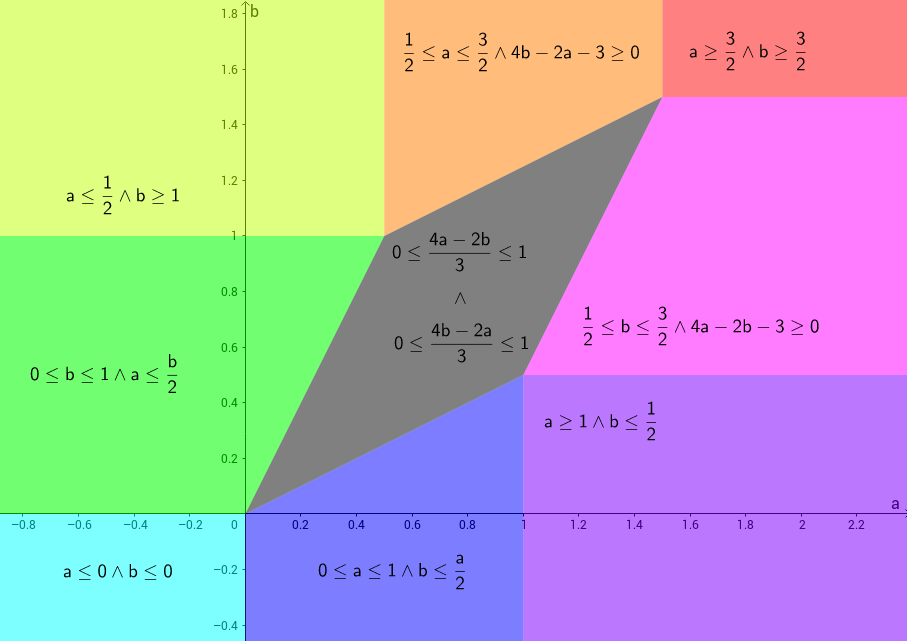
\includegraphics[width=0.9\textwidth]{../Images/a&b_partition.png}
        \caption{Graphical representation of the constraints on \(a\) and \(b\) related to each solution}
        \label{summary-graph}
    \end{figure}
    Moreover, figure \ref{summary-graph} represents all the constraints on \(a\) and \(b\) related to each solution. As you can see, all the possible values of \(a\) and \(b\) have been taken into account and there is no solution which is valid among the same values of \(a\) and \(b\) (except for the values on the edges).
\end{proof}